\begin{figure}[!t]
\centering
\makebox[\linewidth][c]{
\resizebox{\linewidth}{!}{%
\tikzset{
every tree node/.style={align=center,anchor=north}
edge from parent/.style={very thick},
%edge from parent/.style=
%{draw, edge from parent path={(\tikzparentnode.south)
%-- +(0,-8pt)
%-| (\tikzchildnode)}},
blank/.style={draw=none}}
\begin{tikzpicture}[level distance = 30pt]
\fontsize{7}{8}\selectfont{
\matrix (magic) [ampersand replacement=\&]
{
\node{\Tree
    [.All  \edge[blank]; 
    [.Status  \edge[blank];
    [.Party \edge[blank]; 
    [.Mem\# ]]]]};
\&
\node{
    \Tree 
    [.\small{Parliament(2006--2010)}
        [.Government 
            [.$CDA$  $47$ ]
            [.$PvdA$  $37$ ]
            [.$CU$  $6$ ]
        ]
        [.Opposition 
            [.$VVD$  $24$ ]
            [.$PVV$  $10$ ]
            [.$SP$  $27$ ]
            [.$D66$  $3$ ]
            [.$GL$  $10$ ]
        ]
    ]};
\&
\node{
    \Tree 
    [.\small{Parliament(2010--2012)}
        [.Government 
            [.$VVD$  $33$ ]
            [.$CDA$  $23$ ]
        ]
        [.Oppositions
            [.$PvdA$  $32$ ]
            [.$PVV$  $22$ ]
            [.$SP$  $16$ ]
            [.$D66$  $10$ ]
            [.$CU$  $6$ ]
            [.$GL$  $12$ ]
        ]
    ]};
\&
\node{
    \Tree 
    [.\small{Parliament(2012--2014)}
        [.Government 
            [.$VVD$  $43$ ]
            [.$PvdA$  $42$ ]
        ]
        [.Opposition 
            [.$CDA$  $13$ ]
            [.$PVV$  $12$ ]
            [.$SP$  $18$ ]
            [.$D66$  $12$ ]
            [.$CU$  $5$ ]
            [.$GL$  $4$ ]
        ]
    ]};\\
};
}
\end{tikzpicture}
}
}
\caption{Composition of Dutch parliament in 3 periods. \emph{VVD}: People's Party for Freedom and democracy, \emph{PvdA}: Labour Party, \emph{CDA}: Christian Democratic Appeal, \emph{PVV}: Party for Freedom, \emph{SP}: The Socialist Party, \emph{D66}: Democrats 66, \emph{GL}: Green-Left, \emph{CU}: Christian-Union.}
\label{fig:DutchParl}
\end{figure}